\documentclass[final]{fhnwreport}       %[mode] = draft or final
                                        %{class} = fhnwreport, article, 
                                        %          report, book, beamer, standalone
%%---Main Packages-----------------------------------------------------------------------
\usepackage[english, ngerman]{babel}	%Mul­tilin­gual sup­port for LaTeX
\usepackage[T1]{fontenc}				%Stan­dard pack­age for se­lect­ing font en­cod­ings
\usepackage[utf8]{inputenc}				%Ac­cept dif­fer­ent in­put en­cod­ings
\usepackage{lmodern}                    %The newer Font-Set
\usepackage{textcomp}					%LaTeX sup­port for the Text Com­pan­ion fonts
\usepackage{caption}					%Customising captions in floating environments
\usepackage{graphicx} 					%En­hanced sup­port for graph­ics
\usepackage{float}						%Im­proved in­ter­face for float­ing ob­jects
\usepackage{ifdraft}                    %Let you check if the doc is in draft mode
\usepackage{wrapfig}                    %Let wrap text around figures

%%---Useful Packages---------------------------------------------------------------------
\usepackage{color}						%Colour control for LaTeX documents
\usepackage[pdftex,dvipsnames]{xcolor}  %Driver-in­de­pen­dent color ex­ten­sions for LaTeX
\usepackage{csquotes}                   %Simpler quoting with \enquote{}
\usepackage{siunitx} 					%A com­pre­hen­sive (SI) units pack­age
\usepackage{listings}					%Type­set source code list­ings us­ing LaTeX
\usepackage[bottom]{footmisc}			%A range of foot­note op­tions
\usepackage{footnote}					%Im­prove on LaTeX's foot­note han­dling
\usepackage{verbatim}					%Reim­ple­men­ta­tion of and ex­ten­sions to LaTeX ver­ba­tim
\usepackage[textsize=footnotesize]{todonotes} %Mark­ing things to do in a LaTeX doc­u­ment
\usepackage{titling}					%Control over the typesetting of the \maketitle command

%%---Tikz Packages-----------------------------------------------------------------------
\usepackage{standalone}
\usepackage{tikz}
\usepackage{circuitikz}
\usetikzlibrary{arrows}
\usetikzlibrary{calc}
\usetikzlibrary{intersections}

%%---Math Packages-----------------------------------------------------------------------
\usepackage{amsmath}					%AMS math­e­mat­i­cal fa­cil­i­ties for LaTeX
\usepackage{amssymb}					%Type­set­ting symbols (AMS style)
%\usepackage{amstext}
%\usepackage{amsfonts}
%\usepackage{breqn}
\usepackage{array}						%Ex­tend­ing the ar­ray and tab­u­lar en­vi­ron­ments
\usepackage{amsthm}					%Type­set­ting the­o­rems (AMS style)

%%---Table Packages----------------------------------------------------------------------
\usepackage{booktabs}
%\usepackage{vcell}
\usepackage{tabularx}					%Tab­u­lars with ad­justable-width columns
%\usepackage{longtable}
\usepackage{multirow}					%Create tab­u­lar cells span­ning mul­ti­ple rows
\usepackage{makecell}
\usepackage{multicol}					%In­ter­mix sin­gle and mul­ti­ple columns
\usepackage[normalem]{ulem}
\useunder{\uline}{\ul}{}

%%---PDF / Figure Packages---------------------------------------------------------------
\usepackage{pdfpages}					%In­clude PDF doc­u­ments in LaTeX
\usepackage{pdflscape}					%Make land­scape pages dis­play as land­scape
\usepackage{subfig}					    %Fig­ures di­vided into sub­fig­ures

%%---Other Packages----------------------------------------------------------------------
%\usepackage{xargs}                     %De­fine com­mands with many op­tional ar­gu­ments

\lstset{
	aboveskip=1ex,
	backgroundcolor=\color{gray!25},
	basicstyle=\small\ttfamily,
	belowskip=1ex,
	breaklines=true,
	columns=fullflexible,
	framerule=0pt,
	framexrightmargin=0em,
	framexleftmargin=0em,
	numbers=left,
	numberstyle=\footnotesize\sffamily,
	tabsize=2
}

\lstdefinestyle{DOS}
{
	backgroundcolor=\color{black},
	basicstyle=\scriptsize\color{white}\ttfamily
}


%%---Bibliography------------------------------------------------------------------------
\usepackage[style=ieee,urldate=comp,backend=biber]{biblatex}
\addbibresource{literature/bibliography.bib}

%%---Main Settings-----------------------------------------------------------------------
\graphicspath{{./graphics/}}			%Defines the graphicspath
\geometry{twoside=false}				    %twoside=false disables the "bookstyle"
\setlength{\marginparwidth}{2cm}
\overfullrule=5em						%Creates a black rule if text goes over the margins => debugging




%%---User Definitions--------------------------------------------------------------------
%%Tabel-Definitions: (requires \usepackage{tabularx})
\newcolumntype{L}[1]{>{\raggedright\arraybackslash}p{#1}}    %column-width and alignment
\newcolumntype{C}[1]{>{\centering\arraybackslash}p{#1}}
\newcolumntype{R}[1]{>{\raggedleft\arraybackslash}p{#1}}

%%---Optional Package Settings-----------------------------------------------------------
%Listings-Settings: (requires \usepackage{listings}) => Example with Matlab Code
%\lstset{language=Matlab,%
%    basicstyle=\footnotesize\ttfamily,
%    breaklines=false,%
%    morekeywords={switch, case, otherwise},
%    keywordstyle=\color{Blue},%
%    tabsize=2,
%    %morekeywords=[2]{1}, keywordstyle=[2]{\color{black}},
%    identifierstyle=\color{Black},%
%    stringstyle=\color{Purple},
%    commentstyle=\color{Green},%
%    showstringspaces=false,%without this there will be a symbol in the places where there is a space
%    numbers=left,%
%    numberstyle={\tiny \color{black}},% size of the numbers
%    numbersep=9pt, % this defines how far the numbers are from the text
%    %emph=[1]{word1, word2,...},emphstyle=[1]\color{red}
%}							

%Hurenkinder und Schusterjungen verhindern (kein Scherz, Google es)
\clubpenalty10000
\widowpenalty10000
\displaywidowpenalty=10000	


%%---Costum Packages Bachelor Thesis-------------------------------------------
\usepackage{diagbox}

\usepackage{hyperref}
\hypersetup{
    colorlinks=true,
    linkcolor=black,
    filecolor=black,       
    urlcolor=blue,
    citecolor=black,
}			                %loads all packages, definitions and settings
\addbibresource{literature/bibliography.bib}							
\title{Pflichtenheft}  		        %Project Title
\author{Anklin, Bobst, Horath}      				    %Document Type => Technical Report, ...
\date{\today}          				   %Place and Date

\begin{document}

%%---TITLEPAGE---------------------------------------------------------------------------------
\thispagestyle{empty}
%	\ohead{\includegraphics[scale=0.5]{Bilder/Logo_FHNW.jpg}}
	\begin{figure}
		 \vspace*{-\topskip}\vspace*{-\headsep}
		
\includegraphics[scale=1]{graphics/fhnw_ht_logo_de.pdf}
	\end{figure}
	\begin{center}
		\vspace*{2cm}
		{\huge{\textbf{\thetitle}}}\\
		\vspace*{1cm}
		
		{\huge{Testumgebung und Perfomancevergleich von Zigbee, Thread und Bluetooth Mesh Netzwerken}}\\
		\vspace*{0.5cm}
		
		{\scshape\Large Bachelor Thesis - \theauthor \\} \Large{\today}
		\vfill
		
		
		\begin{normalsize}
			{\begin{tabbing}
						
					\textbf{Fachcoach:} \hspace{6cm}\= Matthias Meier\\
					\>Manuel Di Cerbo\\
					
					\\[0.4cm]
					
					\textbf{Team:} \>Raffael Anklin \\ \>Robin Bobst \\ \>Cyrill Horath
					\\[0.8cm]
					\textbf{Studiengang:} \>Elektro- und Informationstechnik
					\\[0.8cm]	\textbf{Semester:} \>Frühlingssemester 2020
			\end{tabbing}}
		\end{normalsize}
		\vfill
	\end{center}
\clearpage


%%---TABLE OF CONTENTS-------------------------------------------------------------------
\pagenumbering{Roman}		
\selectlanguage{ngerman}				%ngerman or english
\tableofcontents
\clearpage

%%---TEXT--------------------------------------------------------------------------------
\pagenumbering{arabic}
	\clearpage
\section{Übersicht}\label{sec:Uebersicht}

Das vorliegende Dokument stellt das Pflichtenheft der Bachelorthesen von Raffael Anklin, Robin Bobst und Cyrill Horath an der Fachhochschule Nordwestschweiz Brugg-Windisch im Studiengang Elektro- und Informationstechnik dar. 
Im kommenden, ersten Kapitel soll eine Übersicht über die Ausgangslage sowie das Ziel dieser Arbeit gegeben werden und somit die Rahmenbedingungen abgesteckt werden. Weiter werden die Lösungskonzepte \ref{sec:Loesungskonzept} sowie die Projektziele und Lieferobjekte \ref{sec:ProjektzieleundLieferobjekte} definiert. Abschliessend soll auch noch das Projektmanagement \ref{sec:Projektmanagement} thematisiert werden. 

\subsection{Ausgangslage}\label{subsec:Ausgangslage}

Unter den standardisierten Low Power Mesh Netzwerk Protokollen im
freien GHz ISM-Band konkurrenzieren sich derzeit vorrangig Bluetooth Mesh, Zigbee sowie Thread.
Bezüglich MAC und Physical Layer basieren Zigbee und Thread auf IEEE 802.15.4 wogegen Bluetooth Mesh auf Bluetooth Low Energy (BLE)
basiert.
Jedes dieser Netzwerkprotokolle hat gewisse Vorzüge: Bluetooth Mesh, dass BLE mittlerweile von jedem Smartphone und Notebook unterstützt wird, Thread aufgrund seiner IPv6 Basis und damit einfachem Übergang ins Internet sowie Zigbee aufgrund seiner etablierten Verbreitung im Smart-Lampenbereich durch Philips, IKEA und Osram.
Hauptproblem aller drei Mesh Netzwerkprotokolle ist nebst physikalisch und distanzbedingter Absorption und Reflexion die Störbeeinflussung durch WLAN (WiFi) und andere Netzwerke im GHz Frequenzbereich.

Im Vorprojekt im Rahmen des P5 mit dem Namen \textit{Bluetooth-Mesh Plattform für IoT Anwendungen} zu dieser Arbeit, wurde das Bluetooth-Mesh Protokoll bereits vertieft betrachtet und dessen Vor- und Nachteile aufgezeigt. Basierend auf diesen Erkenntnissen und Erfahrungen und der oben beschriebenen Thematik soll das Bluetooth-Mesh Protokoll mit den Alternativen Thread sowie Zigbee verglichen werden.

\subsection{Ziel der Arbeit}\label{subsec:ZielderArbeit}

In der vorliegenden Arbeit soll zuerst ein praxistaugliches, einheitliches Testframework für alle drei Mesh Netzwerke erstellt werden, wonach die Tauglichkeit aller drei Mesh Netzwerke unter realitätsnahen Bedingungen ermittelt und verglichen werden soll.
Zwecks besserer Vergleichbarkeit sollen alle drei Testnetze das gleiche Radio-Interface als Grundlage verwenden. Aufgrund der guten
Unterstützung aller drei Mesh Protokolle als auch dem im vergangenen P5 gesammelten Wissens, sollen hierfür die nRF52840 SoCs der Firma Nordic eingesetzt werden. Die zu erstellende Testinfrastruktur soll aus den drei folgenden Teilen bestehen:

\begin{itemize}
 	\item Punkt-Punkt Testinfrastrukturen auf MAC-Ebene
 	\item Test Mesh Netzwerke für BT Mesh, Zigbee und Thread
 	\item Steuer- und Auswertesoftware
\end{itemize}

Die genauen Anforderungen an die Testumgebung sind einerseits in der Aufgabenstellung im Anhang \ref{app:Aufgabenstellung} aufgeführt und andererseits werden sie anhand der Projektziele \ref{sec:ProjektzieleundLieferobjekte} definiert.









\pagebreak

\clearpage
\section{Lösungskonzept}\label{sec:Loesungskonzept}
Zur Messung und Auswertung der Mesh-Netzwerke dient ein Testframework wie es in Abbildung \ref{fig:KonzeptschemaTestframework} schematisch dargestellt ist.

\begin{figure}[H]
	\centering
	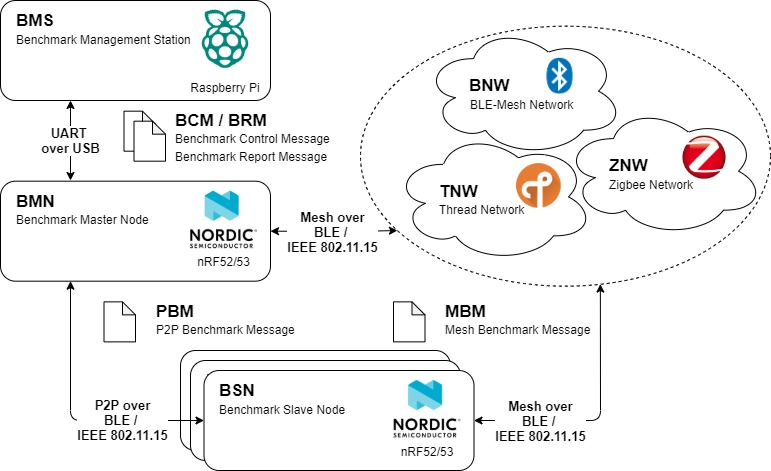
\includegraphics[width=1.0\textwidth]{Konzept_Testframework.jpg}
	\caption{Konzeptschema Testframework}\label{fig:KonzeptschemaTestframework}
\end{figure}


Das Testframework besteht aus folgenden physikalisch getrennten Teilsystemen:

\begin{itemize}
	\item \textbf{BMS} Benchmark Management Station \\ 
	Dient zur Verwaltung und Konfiguration des Testframeworks. Beinhaltet einen Webserver um dem Endanwender die Bedienung zu ermöglichen. Realisiert wird die BMS durch einen \textit{Raspberry Pi 4 Model B}. Als Webserver wird das Python-Framework \textit{Django} eingesetzt. 
	\item \textbf{BMN} Benchmark Master Node \\ 
	Dient als Zugangspunkt der BMS für die im Testframework gefahrenen Tests und lässt sich über eine Serielle Schnittstelle ansprechen. In der Aufgabenstellung \ref{app:Aufgabenstellung} wird der BMN als Master bezeichnet. Realisiert wird der BMN über einen nRF52840 oder nRF5340 von \textit{Nordic}. 
	\item \textbf{BSN} Benchmark Slave Node \\ 
	Dient als Zugriffspunkt der im Testframework gefahrenen Tests und kann frei in der Testumgebung platziert werden. Daher muss die Energieversorgung über einen Akku oder Batterie erfolgen. In der Aufgabenstellung  \ref{app:Aufgabenstellung} wird von einem Slave gesprochen. Realisiert wird der BSN über einen nRF52840 oder nRF5340 von \textit{Nordic}.
\end{itemize}

Die logischen Komponenten des Testframeworks lassen sich wie folgt aufteilen:

\begin{itemize}
	\item \textbf{BCM} Benchmark Control Message \\ 
	Beschreibt Nachrichten welche zur Steuerung eines Benchmarks dienen. Dies sind zum Beispiel Konfigurations-, Start- oder Stop-Befehle. Werden von der BMS initiiert und gelangen über eine USB-UART Verbindung zum BMN. 
	\item \textbf{BRM} Benchmark Report Message \\ 
	Beschreibt Nachrichten welche den Status oder die Ergebnisse eines Benchmarks zurückmelden. Werden vom BMN initiiert und gelangen über eine USB-UART Verbindung zur BMS.
	\item \textbf{PBM} P2P Benchmark Message \\ 
	Nachrichten welche während der Durchführung eines Benchmarks versendet werden. Dies sind zum Beispiel Ping-Anfragen zur Latenzzeitmessung. Sie ermöglichen den Datenaustausch zwischen zwei Teilnehmern auf MAC-Ebene. 
	\item \textbf{MBM} Mesh Benchmark Message \\ 
	Nachrichten welche während der Durchführung eines Benchmarks versendet werden. Dies sind zum Beispiel Ping-Anfragen zur Latenzzeitmessung. Sie ermöglichen den Datenaustausch über ein Mesh-Netzwerk auf Applikations-Ebene. 
\end{itemize}

\subsection{Punkt zu Punkt Testinfrastruktur}\label{subsec:PunktzuPunktTestinfrastruktur}

Der Punkt zu Punkt Benchmark (P2P) soll unabhängig vom Mesh-Protokoll stattfinden. Damit soll es möglich sein die beiden MAC-Ebenen \textit{BLE} und \textit{IEEE802.11.15} zu vergleichen. Der nRF52840 sowie nRF5340 unterstützen das Arbeiten auf der MAC-Schicht. Zur Realisierung wird ein bereits bestehendes Beispiel (Radio-Example) aus der nRF Connect SDK genutzt.


\subsection{Test Mesh Netzwerke}\label{subsec:TestMeshNetzwerke}

Der Mesh-Benchmark soll die verschiedenen Mesh-Netzwerke möglichst identisch ausmessen. Dazu dient bei allen Mesh-Netzwerken die Applikations-Schicht. Ein Mesh Netzwerk wird zwischen dem BMN und den BSN aufgebaut. Dazu werden die einzelnen Nodes über die BMS mit der entsprechenden Firmware geladen und anschliessend im Raum verteilt. Das Laden ist zu Beginn über eine Kabelverbindung (UART) vorgesehen. Zu einem späteren Zeitpunkt soll dies drahtlos mithilfe eines Bootloaders möglich gemacht werden. 

\subsubsection{Bluetooth Mesh}\label{subsubsection:Bluetooth Mesh}

Die BLE-Mesh Firmware der Nodes werden aus Beispielen der nRF Connect SDK und Zephyr abgeleitet. Das Mesh-Demo Beispiel erlaubt es die essentiellen Netzwerk Parameter fix vorzugeben. Dadurch müssen die Nodes nicht mehr Provisioniert werden und sind sofort einsatzbereit.

\newpage
\subsubsection{Thread}\label{subsubsection:Thread} 
Die Abbildung \ref{fig:ThreadKonzept} zeigt das Framework des Openthread Netzwerkes auf. Die BMS kommuniziert via UART mit dem wpantund Protokoll von Google. Die Daten zum NCP, welcher auf dem BMN realisiert wird, werden mit Hilfe von Spinel übertragen. Der BMN sendet die erhaltenen Daten danach in das Thread Netzwerk.

\begin{figure}[H]
	\centering
	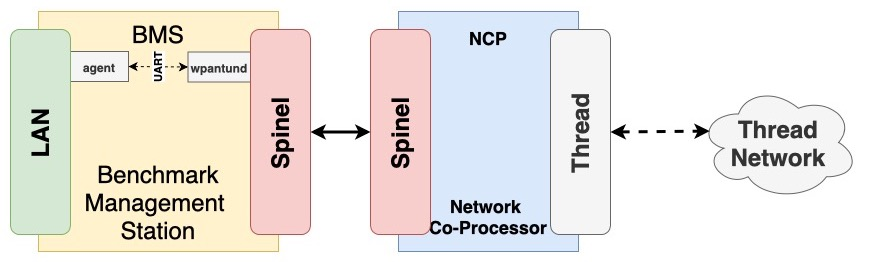
\includegraphics[width=1.0\textwidth]{Thread-Konzept.jpg}
	\caption{Konzept OpenThread Framework}\label{fig:ThreadKonzept}
\end{figure}



\subsubsection{Zigbee}\label{subsubsection:Zigbee}
Das Zigbee Test Mesh Netzwerk wird mithilfe der \textit{nRF SDK for Thread and Zigbee} eingerichtet und für die Messungen vorbereitet. Der BMN wird dabei als Zigbee Coordinator und gleichzeitig als Zigbee Router eingesetzt. Die BSN können wieder als Router oder aber als Zigbee End Device betrieben werden.


\subsection{Steuer und Auswertesoftware}\label{subsec:SteuerundAuswertesoftware}
Die Steuerung des Testframeworks erfolgt über eine Weboberfläche. Diese wird von der BMS mittels WLAN auf den Benutzergeräten zur Anzeige gebracht. Als Webserver dient das Python-Framework \textit{Django}. Zur Steuerung der Benchmarks dienen Schrittketten, welche mit der Firmware auf dem BMN kommunizieren. Als letzter Schritt eines Benchmarks werden die Ergebnisse geloggt, nachbearbeitet und wiederum zur Anzeige gebracht.


\pagebreak

\clearpage
\section{Projektziele und Lieferobjekte}\label{sec:ProjektzieleundLieferobjekte}

Nachfolgend sind alle Projektziele aufgelistet. Die Ziele wurden in drei verschiedene Themen aufgeteilt.

\subsection{Punkt zu Punkt Testinfrastruktur}\label{subsec:PunktzuPunktTestinfrastruktur}

\begin{table}[H]
	\begin{tabular}{ | C{0.7cm} | p{2.8cm} | p{8.2cm} | C{2.5cm} |}
		\hline
		\multicolumn{4}{|l|}{\textbf{Projektziele}}\\ \hline
		\textbf{Nr.}& \textbf{Ziel}& \textbf{Beschrieb}& \textbf{\begin{tabular}[b]{@{}c@{}}Pflicht- oder\\Wunschziel\end{tabular}}\\ \hline
		
		P1 & Kommunikation mit BMS & Das BMN kommuniziert via USB oder UART mit dem BMS.  & Pflichtziel\\ \hline
		
		P2 & Absenden von MAC-Frames & Das BMN sendet gemäss den Vorgaben des BMS regelmässig MAC-Frames an einen oder mehrere BSN. & Pflichtziel\\ \hline
		
		P3 & Rückbestätigung der MAC-Frames & Der oder die batteriebetriebenen BSN, bestätigen die MAC-Frames zurück. & Pflichtziel\\ \hline
		
		P4 & Konfiguration der Anzahl BSN & Die Anzahl der BSN ist über eine Steuer- und Auswertesoftware konfigurierbar. & Pflichtziel\\ \hline
		
		P5 & Konfiguration der ID der BSN & Die ID der BSN ist über eine Steuer- und Auswertesoftware konfigurierbar. & Pflichtziel\\ \hline
		
		P6 &Konfiguration der Kanäle & Die BLE resp. 802.15.4 Kanäle können über eine Steuer- und Auswertesoftware ausgewählt werden. & Pflichtziel\\ \hline
		
		P7 & Einstellbare Framelänge & Die Framelänge der MAC-Frames ist über eine Steuer- und Auswertesoftware konfigurierbar. & Pflichtziel\\ \hline
		
		P8 & Einstellbare Frame- und Kanalwechselrate& Die Frame- und Kanalwechselrate der BSN ist über eine Steuer- und Auswertesoftware konfigurierbar. & Pflichtziel\\ \hline
		
		P9 & Einstellbare Sendeleistung & Die Sendeleistung der BSN ist über eine Steuer- und Auswertesoftware konfigurierbar. & Pflichtziel\\ \hline
		
		P10 & Anpassung der Modulationsart& In BLE soll die Modulationsart über eine Steuer- und Auswertesoftware konfigurierbar sein, um die Datenrate von 125kbps auf 2Mbps und die Long Range Funktion einzustellen. & Pflichtziel\\ \hline
		
		P11 & Ein- und Ausschalten der Collision Avoidance (CSMA/CA)& Beim 802.15.4 Protokoll soll die Collision Avoidance über eine Steuer- und Auswertesoftware ein- und ausgeschaltete werden können. & Pflichtziel\\ \hline
		
		P12 & Erfassen der Verbindungsqualität & Sowohl master- wie auch slaveseitige Erfassung der Verbindungsqualität (RSSI, Package Loss, Collisions, Noise Level, …). Die BSN senden hierzu die erfassten Werte im Rückantwortframe dem BMN zurück. & Pflichtziel\\ \hline
		
		W1 & Testmodul BMN/BSN & Entwickeln einer Hardware mit unabhängiger Stromversorgung und dezidierter Strommessung, um den Stromverbrauch aufzuzeichnen. \\ \hline
		
	\end{tabular}\\
	\caption{Projektziele der Punkt zu Punkt Testinfrastruktur}
	\label{tab:ProjektzielederPunktzuPunktTestinfrastruktur}
\end{table}


\subsection{Test Mesh Netzwerke}\label{subsec:TestMeshNetzwerke}
\begin{table}[H]
	\begin{tabular}{ | C{0.7cm} | p{2.8cm} | p{8.2cm} | C{2.5cm} |}
		\hline
		\multicolumn{4}{|l|}{\textbf{Projektziele}}\\ \hline
		\textbf{Nr.}& \textbf{Ziel}& \textbf{Beschrieb}& \textbf{\begin{tabular}[b]{@{}c@{}}Pflicht- oder\\Wunschziel\end{tabular}}\\ \hline
		
		P1 & Kommunikation mit BMS & Das BMN kommuniziert via USB oder UART mit dem BMS. & Pflichtziel\\ \hline
		
		P2 &Konfiguration BSN &Die BSN lassen sich frei zu einem Routing-Knoten, End-Knoten oder einem Low-Power Knoten konfigurieren. & Pflichtziel\\ \hline
		
		P3 & Mesh-Netzwerk & Alle drei Technologien Bluetooth, Thread und Zigbee müssen als Mesh-Netzwerk mit mindestens 10 BSN aufgebaut werden. & Pflichtziel\\ \hline
		
		P4 & Simulation Sensorwerte & Die BSN sollen in einem vom BMS vorgegebenen parametrisierbaren Intervall Sensorwerte Simulieren& Pflichtziel\\ \hline
		
		P5 & Sensordaten & Als Sensordaten sollen die Netzzustandsdaten übermittelt werden: Paketnummer, Anzahl Retries, Paketverluste, RSSI, Strombedarf und aktive CPU- und Radio-Zeiten. & Pflichtziel\\ \hline
		
		P6 & Störimmunität & Um die Störimmunität der Netzwerke zu ermitteln sollen gezielt Fremdstörungen mit eingebracht werden, mit definierbarer Tastung und Störframelänge. Hierfür sollen die Punkt zu Punkt Testinfrastrukturen auf MAC-Ebene eingesetzt werden & Pflichtziel\\ \hline
		
		P7 & Test und Validierung & Umfassende Gegenüberstellung und Validierung aller drei Netzwerke in einem FHNW Gebäude, insbesondere Durchsatz, Antwortzeit, Zuverlässigkeit, Einfachheit der Konfiguration (inkl. Routing), Einfachheit der Ermittlung geeigneter Router-Standorte, Sicherheit und Energieverbrauch. & Pflichtziel\\ \hline
		
	\end{tabular}\\
	\caption{Projektziele der Test Mesh Netzwerke}
	\label{tab:ProjektzielederTestMeshNetzwerke}
\end{table}


\subsection{Steuer- und Auswertesoftware}\label{subsec:SteuerundAuswertesoftware}
\begin{table}[H]
	\begin{tabular}{ | C{0.7cm} | p{2.8cm} | p{8.2cm} | C{2.5cm} |}
		\hline
		\multicolumn{4}{|l|}{\textbf{Projektziele}}\\ \hline
		\textbf{Nr.}& \textbf{Ziel}& \textbf{Beschrieb}& \textbf{\begin{tabular}[b]{@{}c@{}}Pflicht- oder\\Wunschziel\end{tabular}}\\ \hline
		
		P1 & Ansteuerung Funkmodul & Das BMS steuert via USB oder UART ein BMN an.  & Pflichtziel\\ \hline
		
		P2 & Visualisierung Parameter& Die Parameter der Ziele von Kapitel \ref{subsec:TestMeshNetzwerke} und \ref{subsec:PunktzuPunktTestinfrastruktur} sollen vom BMS visualisiert und eingestellt werden können. & Pflichtziel\\ \hline
		
		P3 & Konfiguration Mesh-Netzwerk& Das BMS verwaltet und konfiguriert über einen BMN das Mesh-Netzwerk. & Pflichtziel\\ \hline
		
		P4 & Einheitliche Kommunikation von BMS & Das Protokoll und Interface zum BMS soll für alle drei Mesh-Netzwerke einheitlich sein & Pflichtziel\\ \hline
		
	\end{tabular}\\
	\caption{Projektziele der Steuer- und Auswertesoftware}
	\label{tab:ProjektzielederSteuerundAuswertesoftware}
\end{table}


\subsection{Lieferobjekte}\label{subsec:Lieferobjekte}
Zusätzlich zu den Projektzielen, folgen in diesem Kapitel die Lieferobjekte  mit dem jeweiligen Fälligkeitsdatum. In der Tabelle \ref{tbl:Lieferobjekte} sind diese  aufgelistet.  


\begin{table}[H]
     \centering
\begin{tabular}{|c|c|l|}\hline
   \textbf{Nr.} & \textbf{Datum} & \textbf{Lieferobjekt} \\ \hline
   
   1 & 02.03.2020 & Abgabe Pflichtenheft, 1. Version\\ \hline
   2 & 08.03.2020 & Abgabe Pflichtenheft, definitive Version\\ \hline
   3 & 14.08.2020 & Abgabe Fachbericht \\ \hline
   4 & 14.08.2020 & Abgabe Paper \\ \hline
   5 & 14.08.2020 & Abgabe Testaufbau \\ \hline
   6 & 14.08.2020 & Abgabe Factsheet \\ \hline
   7 & 14.08.2020 & Abgabe Poster \\ \hline
   8 & 01.09.2020 & Projektpräsentation \\ \hline
   
 \end{tabular}
     \caption{Lieferobjekte}
     \label{tbl:Lieferobjekte}
\end{table}
\pagebreak

\clearpage
\section{Projektmanagement}\label{sec:Projektmanagement}
\todo[inline]{Cyrill}

\todo[inline]{Schlankes Projektmanagement mit Projektplan im Anhang. 3 Teile einzeln plus ein Teil gemeinsam.} 
\todo[inline]{Alle 2 Wochen soll eine Projektsitzung mit den Dozenten abgehalten werden.}

Nachfolgend werden die wichtigsten Punkte bezüglich Projektmanagement behandelt. Dieses Kapitel wird bewusst so klein als möglich gehalten, sodass jedoch die wichtigsten Eckpunkte definiert sind.

\subsection{Projektaufteilung}\label{subsec:Projektaufteilung}
\todo[inline]{Cyrill}

\todo[inline]{Evtl. Tabelle mit Definition der Aufteilung. Wer ist für welchen Teil zuständig.}

Wie bereits im Kapitel \ref{sec:Uebersicht} erwähnt, stellt die vorliegende Projektarbeit die Bachelorthesen von Raffael Anklin, Robin Bobst und Cyrill Horath dar. Die einzelnen Thesen werden grundsätzlich als separate Projekte behandelt welche jedoch einen gemeinsamen Teil beinhalten. Innerhalb dieses gemeinsame Teils welcher als Framework bezeichnet wird, werden die Arbeitspakete dynamisch an die 3 Mitarbeiter verteilt. In der Tabelle \ref{tab:ZuweisungderZustaendigkeiten} ist die genaue Zuweisung der Zuständigkeiten ersichtlich.

\begin{table}[H]
     \centering
     	\begin{tabular}{ | p{2.5cm} | p{6cm} | p{2.7cm} | C{2.8cm} |}\hline
  		\textbf{Bezeichnung} & \textbf{Inhalt} & \textbf{Zuständigkeit} & \textbf{Kennung} \\ \hline
   
   Bluetooth Mesh & Aufbau, Messung und Analyse eines Bluetooth Mesh Netzwerks & Raffael Anklin & EIT-P-20FS-030\\ \hline
   Thread & Aufbau, Messung und Analyse eines Thread Mesh Netzwerks & Robin Bobst & EIT-P-20FS-031\\ \hline
   Zigbee & Aufbau, Messung und Analyse eines Zigbee Mesh Netzwerks & Cyrill Horath & EIT-P-20FS-032 \\ \hline
   Framework & Bereitstellung der Test- und Messinfrastruktur. & Alle & - \\ \hline
   
 \end{tabular}
     \caption{Zuweisung der Zuständigkeiten}
     \label{tab:ZuweisungderZustaendigkeiten}
\end{table}





\subsection{Projektplan}\label{subsec:Projektplan}
\todo[inline]{Framework --> Raffi}
\todo[inline]{Einzelprojekte der jeweils Zuständige}

\todo[inline]{Projektpläne erstellen}
\todo[inline]{Verweis auf die Projektpläne Framework und 3 mal Mesh Netzwerke.}

\subsection{Risikoanalyse}\label{subsec:Risikoanalyse}
\todo[inline]{Robin: Risikoanalyse erstellen und in den Anhang einfügen}




\subsection{Projektvereinbarung}\label{subsec:Projektvereinbarung}

	\begin{tabbing}
		\textbf{Projektcoach}\\[0.2cm]
		Di Cerbo Manuel\\[0.2cm]
		Ort, Datum: \hspace{5cm}\=Unterschrift:
		\\[0.5cm]----------------------------- \>-----------------------------
		\\[0.2cm]
		Meier Matthias\\[0.2cm]
		Ort, Datum: \hspace{5cm}\=Unterschrift:
		\\[0.5cm]----------------------------- \>-----------------------------
		\\[1cm]
		\textbf{Projekt: EIT-P-20FS-030}\\[0.2cm]
		Anklin Raffael\\[0.2cm]
		Ort, Datum: \>Unterschrift:
		\\[0.5cm]----------------------------- \>-----------------------------
		\\[0.2cm]
		\textbf{Projekt: EIT-P-20FS-031}\\[0.2cm]		
		Bobst Robin\\[0.2cm]
		Ort, Datum: \>Unterschrift:
		\\[0.5cm]----------------------------- \>-----------------------------
		\\[0.2cm]
		\textbf{Projekt: EIT-P-20FS-032}\\[0.2cm]
		Horath Cyrill\\[0.2cm]
		Ort, Datum: \>Unterschrift:
		\\[0.5cm]----------------------------- \>-----------------------------
	\end{tabbing}
	
	\clearpage
\pagebreak



\clearpage
%%---BIBLIOGRAPHY------------------------------------------------------------------------
{\sloppypar
\printbibliography[heading=bibintoc]
\label{sec:lit}
%\selectlanguage{ngerman}				%ngerman or english
%\printbibliography
}

%%---APPENDIX----------------------------------------------------------------------------
\begin{appendix} 

\addcontentsline{toc}{section}{Anhang}


%**********************Aufgabenstellung***************************
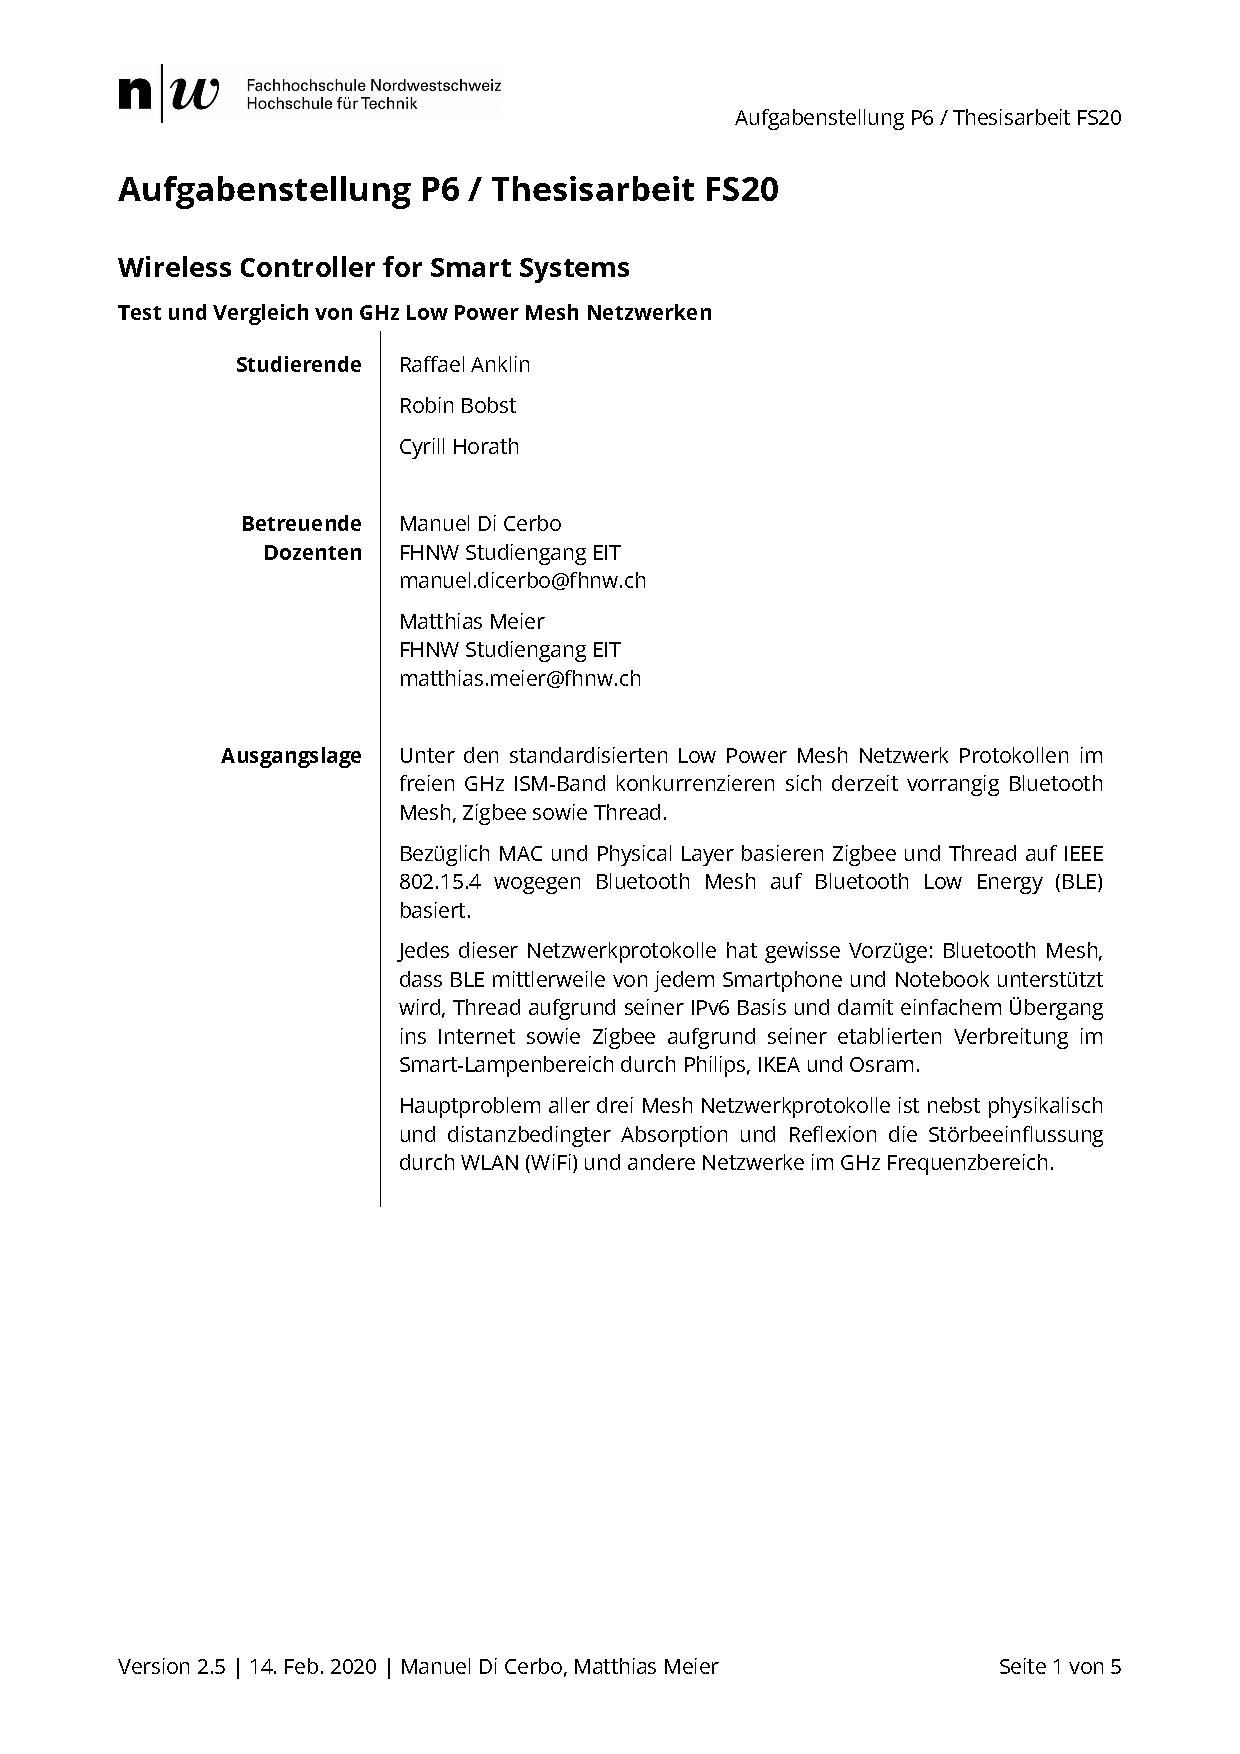
\includepdf[pages={1}, nup=1x1, landscape=false, scale=0.9 ,offset=0 -45, pagecommand={\section{Aufgabenstellung}\label{app:Aufgabenstellung}\thispagestyle{myheadings}}]{appendix/P6_Aufgabenstellung_Wireless_Controller_for_Smart_Systems.pdf}

\includepdf[pages={2-5}, nup=1x1, landscape=false, scale=0.9 ,offset=0 -45, pagecommand={\thispagestyle{myheadings}}]{appendix/P6_Aufgabenstellung_Wireless_Controller_for_Smart_Systems.pdf}


%**********************Pflichtenheft***************************

\includepdf[pages={1}, nup=1x1, landscape=false, scale=0.95 ,offset=0 -45, pagecommand={\section{Pflichtenheft}\label{app:Pflichtenheft}\thispagestyle{myheadings}}]{appendix/P6_Pflichtenheft.pdf}


\includepdf[pages={2-19}, nup=1x1, landscape=false, scale=0.95 ,offset=0 -45, pagecommand={\thispagestyle{myheadings}}]{appendix/P6_Pflichtenheft.pdf}

%***************EMV Bericht Abstrahlung Antennen*********************
\includepdf[pages={1}, nup=1x1, landscape=false, scale=0.95 ,offset=0 -45, pagecommand={\section{Bericht emv Messung Development Kits}\label{app:BerichtemvMessungDevelopmentKits}\thispagestyle{myheadings}}]{appendix/emv_Bericht_FS20.pdf}

\includepdf[pages={2-13}, nup=1x1, landscape=false, scale=0.95 ,offset=0 0, pagecommand={\thispagestyle{myheadings}}]{appendix/emv_Bericht_FS20.pdf}

%***************Messprotokolle Mesh Benchmark*********************
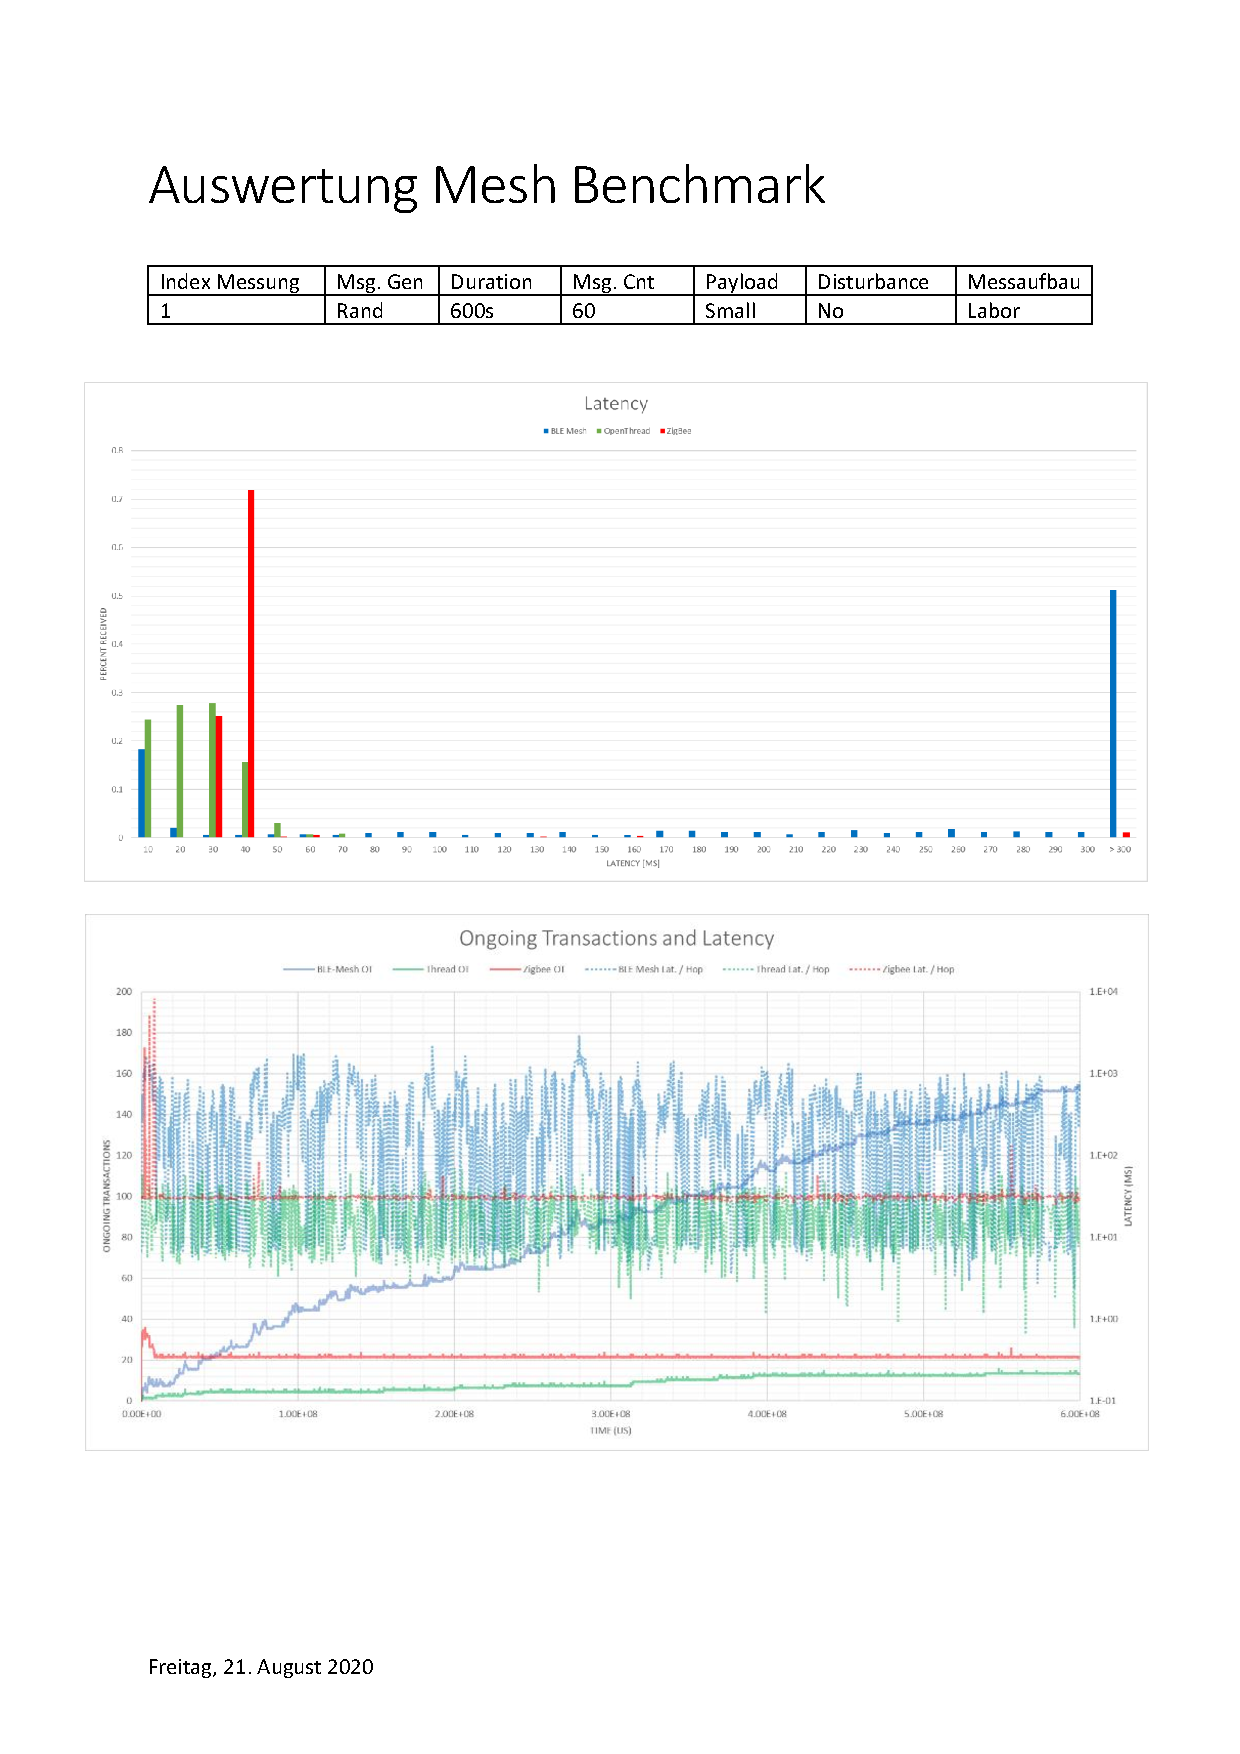
\includepdf[pages={1}, nup=1x1, landscape=false, scale=0.95 ,offset=0 -20, pagecommand={\section{Messprotokolle Mesh Benchmark}\label{app:MessprotokolleMeshBenchmark}\thispagestyle{myheadings}}]{appendix/Messprotokolle_Labor.pdf}

\includepdf[pages={2-14}, nup=1x1, landscape=false, scale=0.95 ,offset=0 0, pagecommand={\thispagestyle{myheadings}}]{appendix/Messprotokolle_Labor.pdf}

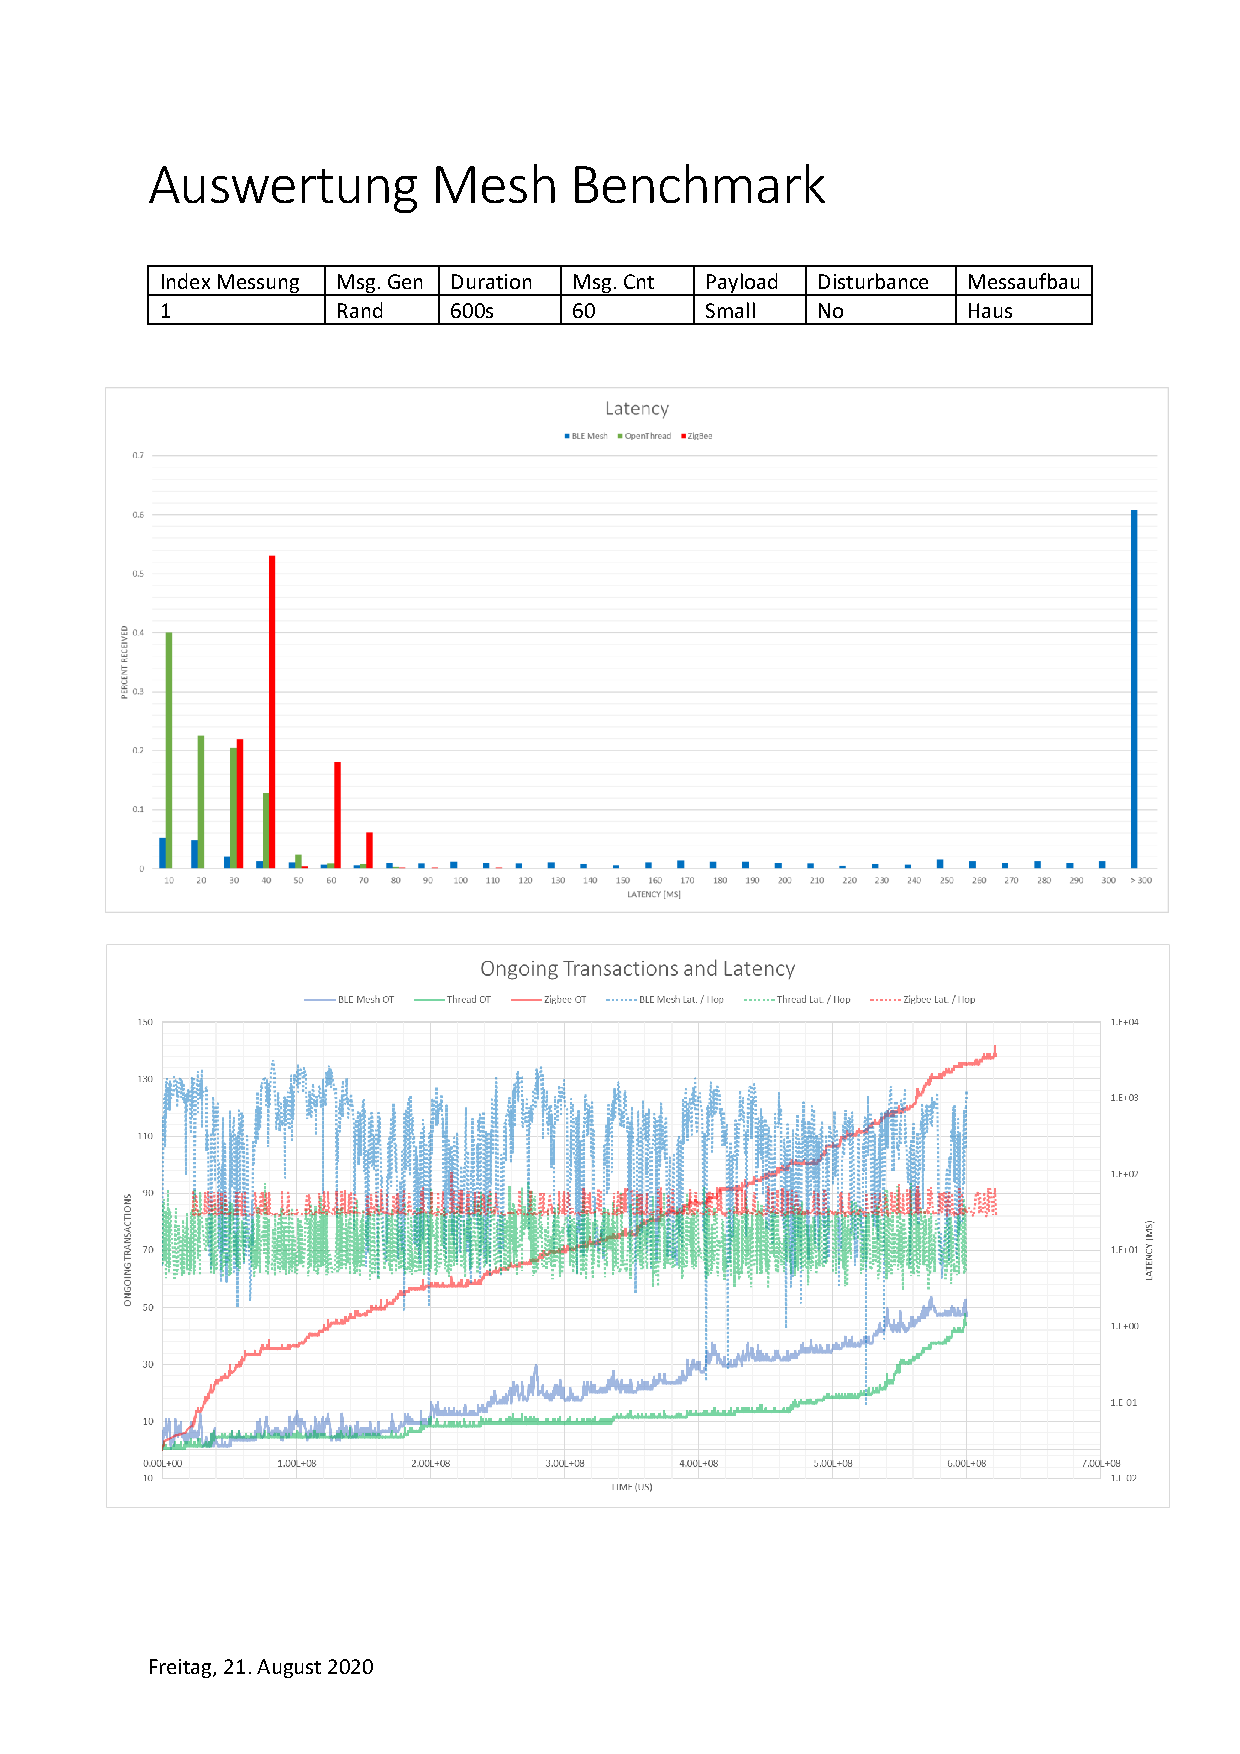
\includepdf[pages={1}, nup=1x1, landscape=false, scale=0.95 ,offset=0 0, pagecommand={\thispagestyle{myheadings}}]{appendix/Messprotokolle_Haus.pdf}

\includepdf[pages={2-8}, nup=1x1, landscape=false, scale=0.95 ,offset=0 0, pagecommand={\thispagestyle{myheadings}}]{appendix/Messprotokolle_Haus.pdf}

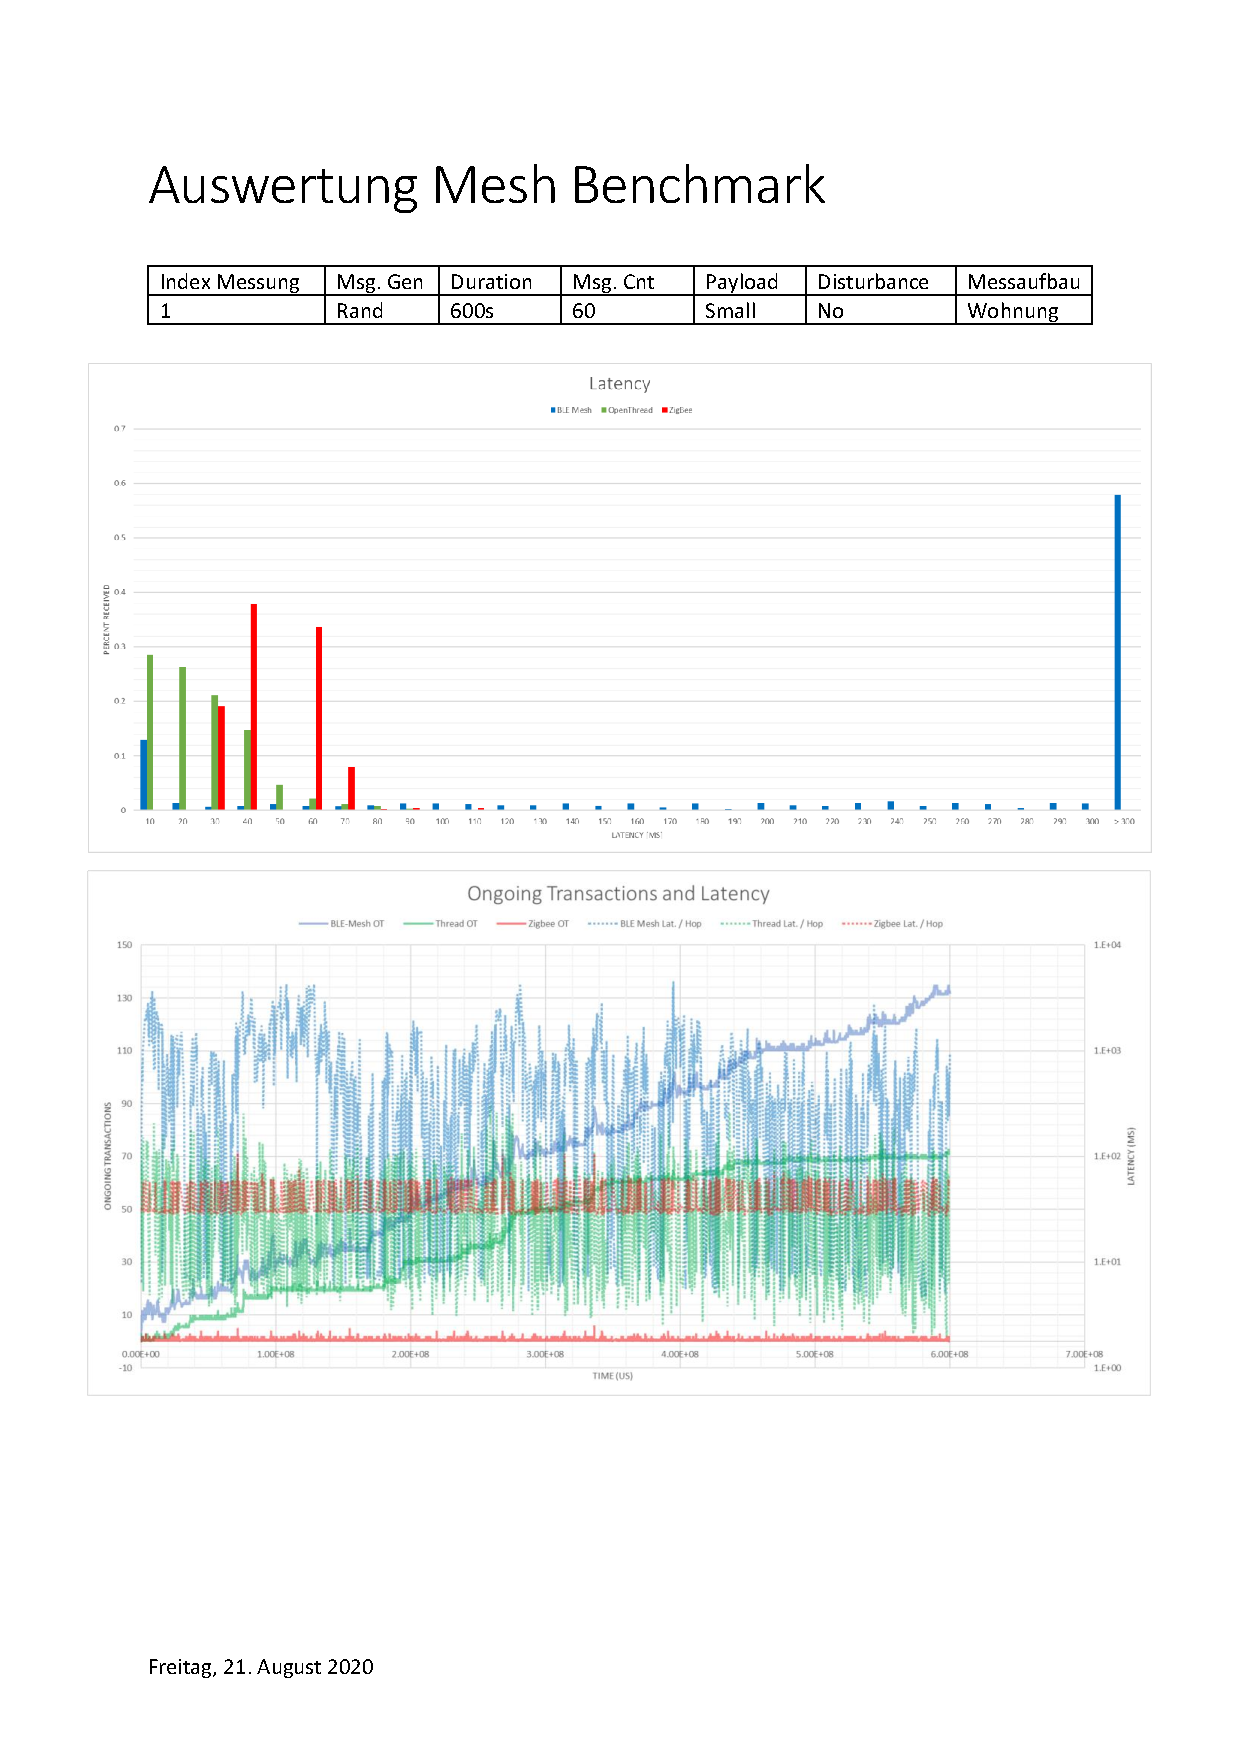
\includepdf[pages={1}, nup=1x1, landscape=false, scale=0.95 ,offset=0 0, pagecommand={\thispagestyle{myheadings}}]{appendix/Messprotokolle_Wohnung.pdf}

\includepdf[pages={2-8}, nup=1x1, landscape=false, scale=0.95 ,offset=0 0, pagecommand={\thispagestyle{myheadings}}]{appendix/Messprotokolle_Wohnung.pdf}

%***************Random Value Generation*********************
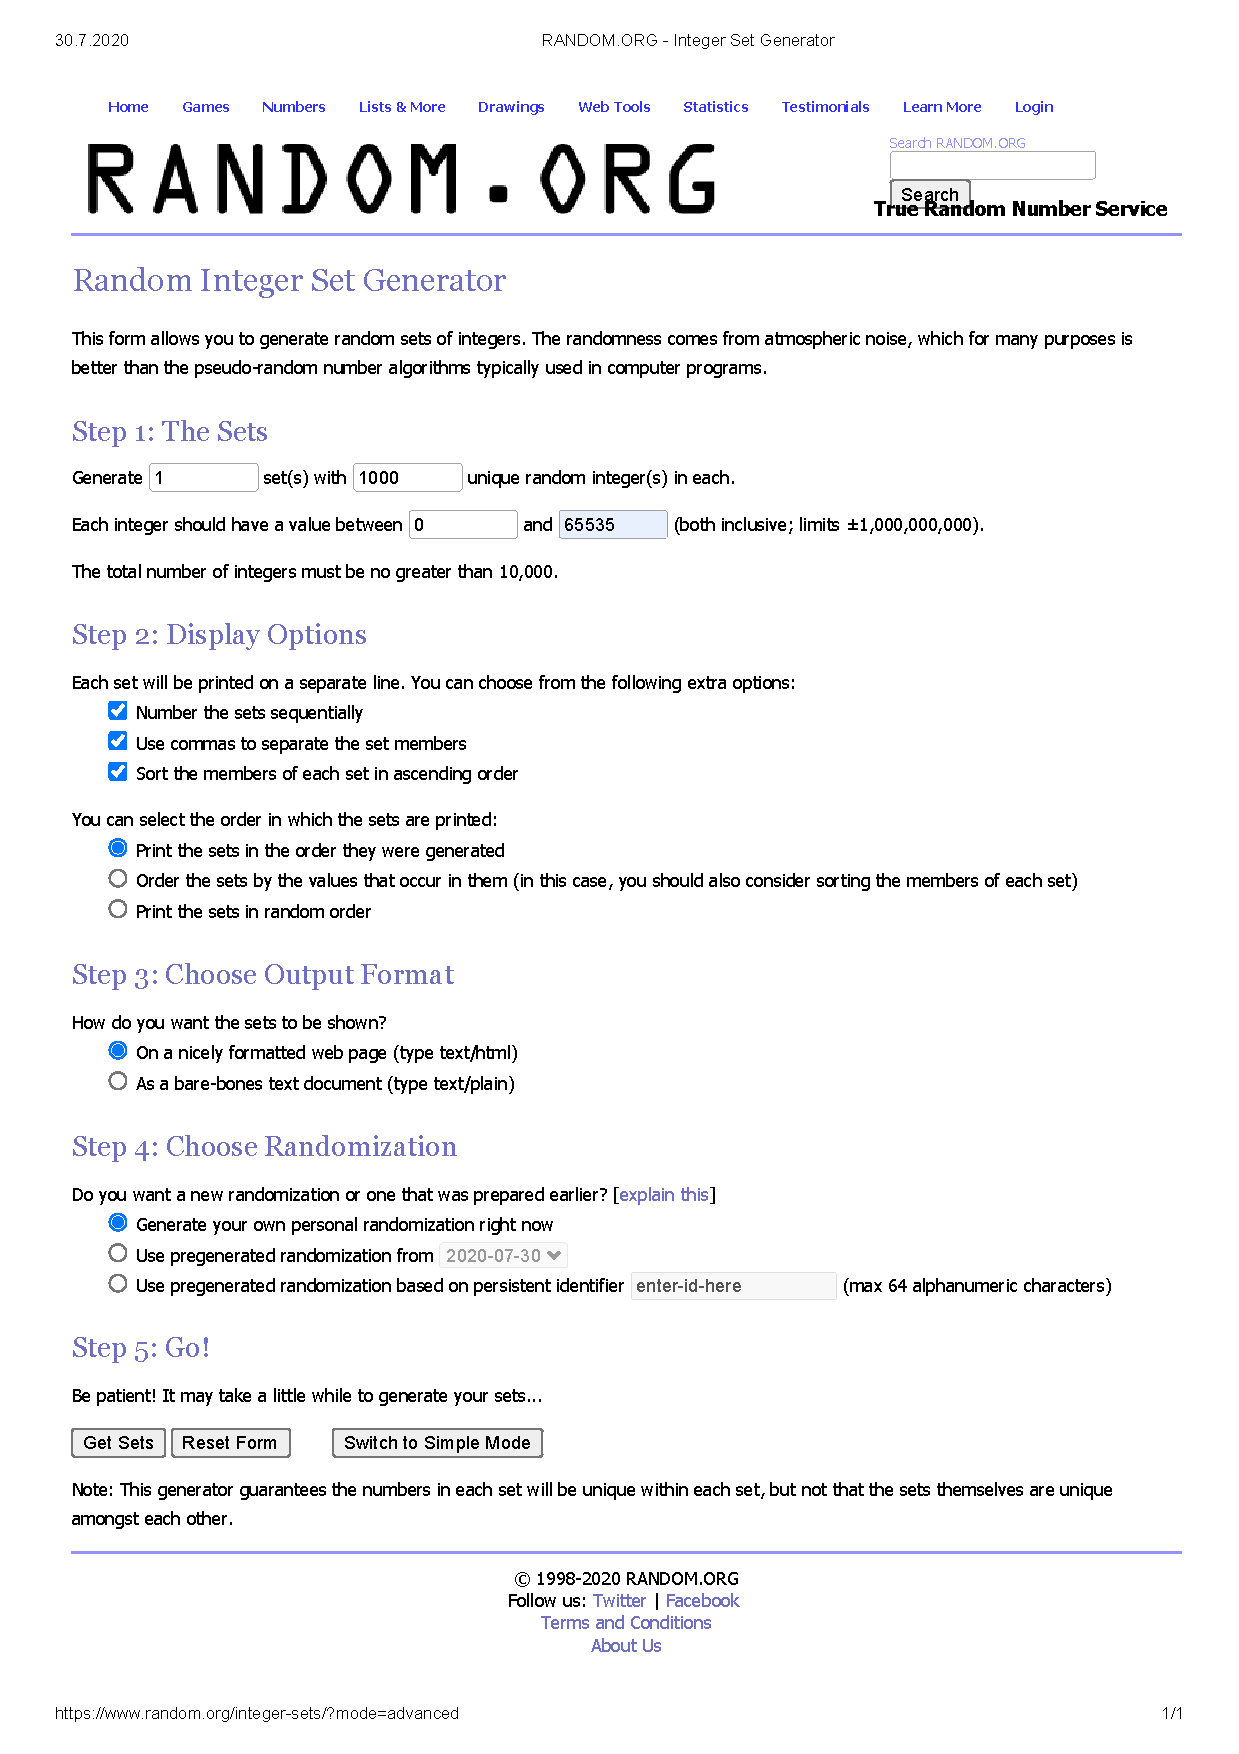
\includepdf[pages={1}, nup=1x1, landscape=false, scale=0.8 ,offset=0 -20, pagecommand={\section{Random Traffic Generation}\label{app:RandomTrafficGeneration}\thispagestyle{myheadings}}]{appendix/RANDOM.ORG_Integer_Set_Generator.pdf}


\end{appendix}



%%---NOTES for DEBUG---------------------------------------------------------------------
\ifdraft{%Do this only if mode=draft
%%requires \usepackage{todonotes})
\newpage
\listoftodos[\section{Todo-Notes}]
\clearpage
}
{%Do this only if mode=final
}

\end{document}
